\section{Aim}

Keywords, that are giving the most portion of the overall sales are usually tracked for visibility. These keywords are updated using the visibility rules. The rules for visibility are pretty simple, using only the current rank and the desired rank.

\section{Assumptions}

\begin{enumerate}
    \item The placement of a target depend on the bid. Higher the bid, the higher the placement.
    \item Increasing bids results in higher placement and decreasing bids results in lower placement.
\end{enumerate}

\section{Visibility Rules}

The rules are simple. We just compare the desired rank with the current rank and increase or decrease the bid based on the difference between the two. We use the average CPC of the whole category for this. The following figure shows the rules.

\subsection{get\_visible\_keywords Function}

\begin{lstlisting}[language=Python]
def get_visible_keywords(client_profile_id):
    # ... (code omitted for brevity)
    return visible_keywords
\end{lstlisting}

This function retrieves a list of keywords that are visible and creates a list of ASINs (Amazon Standard Identification Numbers) that are visible with the keyword. The function takes as input a string `client\_profile\_id` which is the client profile id of the client.

The function first constructs a SQL query to retrieve the distinct keywords, ASINs, campaign IDs, and campaign types from the `visibility\_clean` table where the `client\_profile\_id` matches the input and the date is greater than the current date minus 1.

The function then runs the query and retrieves the data into a DataFrame `visibility\_df`. It then groups the data by `Targeting` and `campaignType\_v` and aggregates the `asin` and `campaignId\_v` columns using a custom aggregation function `agg\_function`.

Finally, the function renames the columns of the DataFrame and returns it.

\subsection{get\_asin\_visible\_precentage Function}

\begin{lstlisting}[language=Python]
def get_asin_visible_precentage(target_asins, visible_asins):
    # ... (code omitted for brevity)
    return len(intersection) / len(target_asins)
\end{lstlisting}

This function calculates the percentage of ASINs that are visible for a keyword. The function takes as input two strings `target\_asins` and `visible\_asins` which are the ASINs that are targeted and the ASINs that are visible, respectively.

The function first checks if `target\_asins` or `visible\_asins` is null. If either is null, it returns 0. If neither is null, it splits `target\_asins` and `visible\_asins` into lists.

The function then finds the intersection of the `target\_asins` and `visible\_asins` lists and calculates the length of the intersection divided by the length of `target\_asins`. This is the percentage of ASINs that are visible. The function then returns this percentage.


\subsection{Flow Chart for Visibility Rules}

The \ref{fig:visibility_bids} shows the flow chart for the visibility rules.
\begin{figure}[ht]
    \centering
    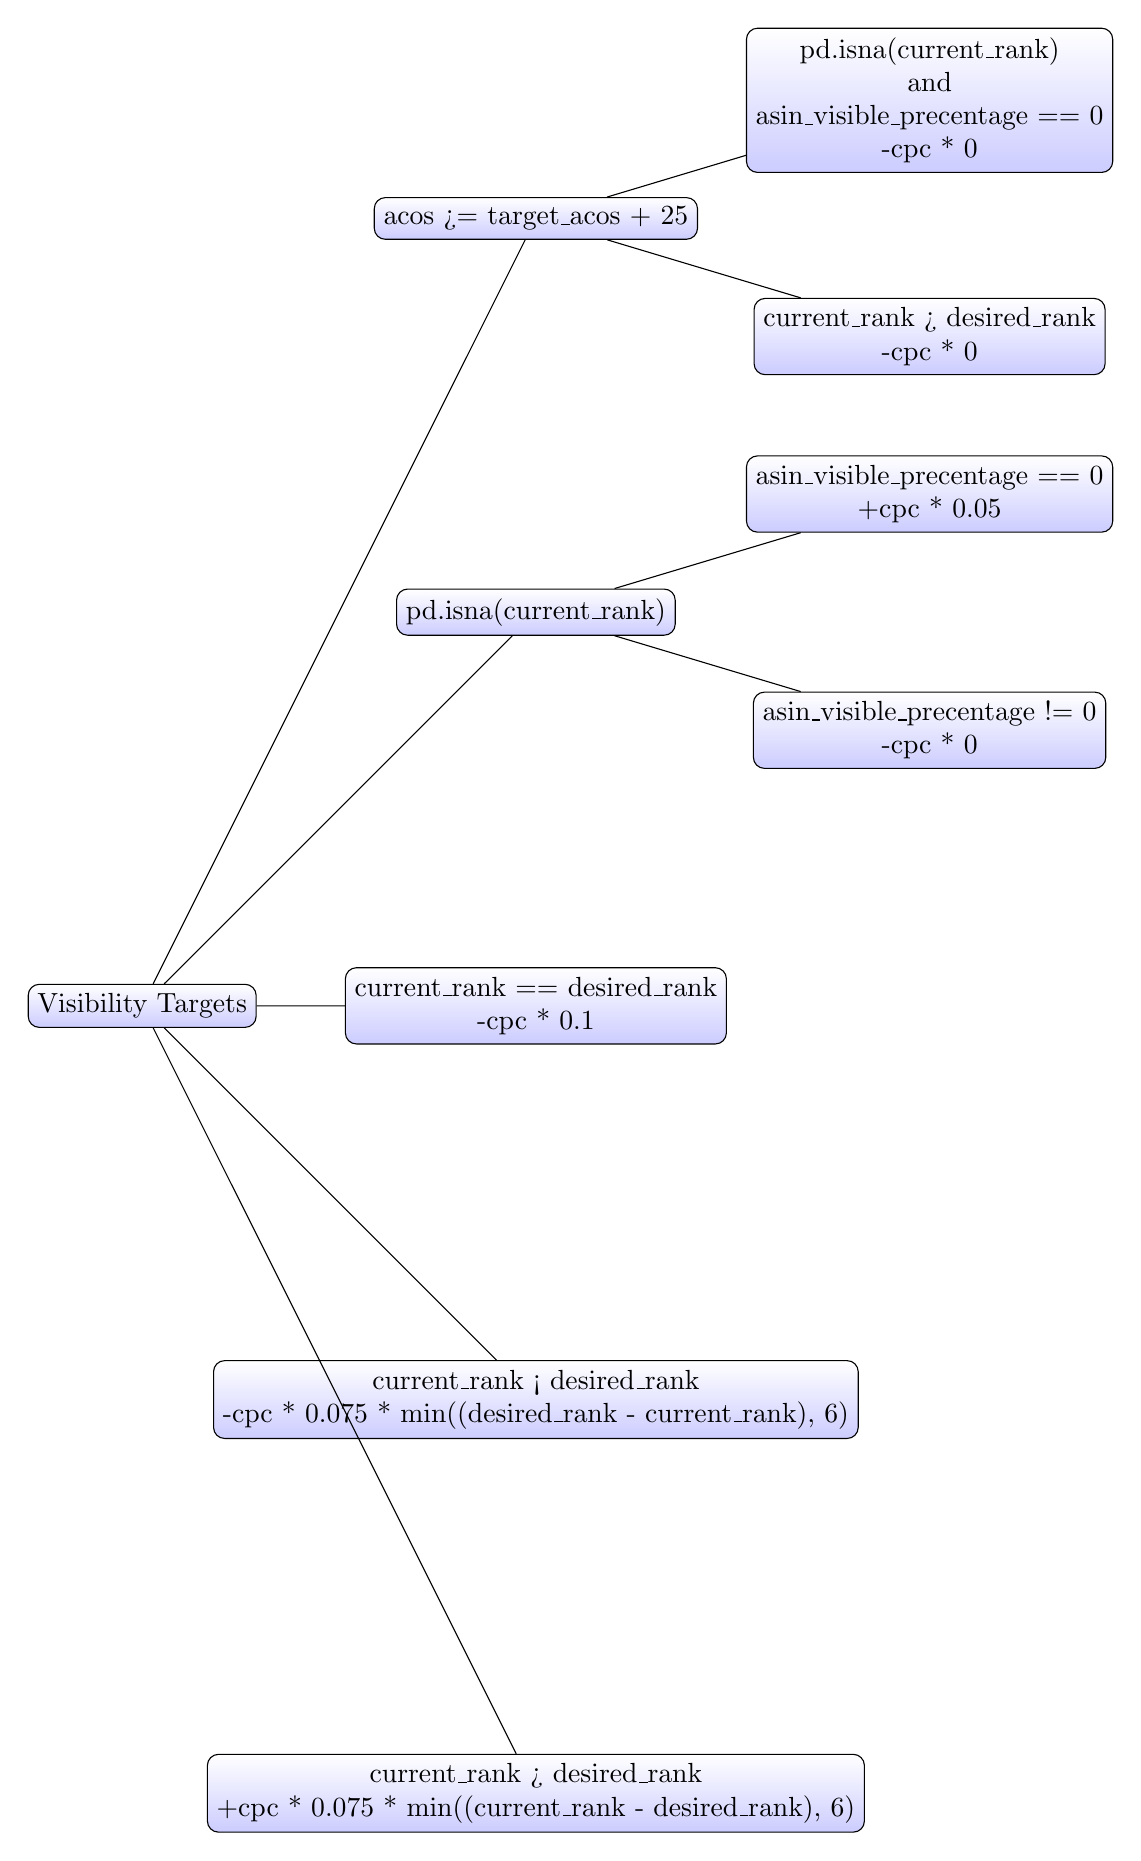
\begin{tikzpicture}[
            grow'=right,
            level 1/.style={level distance=5cm, sibling distance=5cm},
            level 2/.style={level distance=5cm, sibling distance=3cm},
            every node/.style = {shape=rectangle, rounded corners, draw, align=center, top color=white, bottom color=blue!20}
        ]

        \node {Visibility Targets}
        child { node {acos >= target\_acos + 25}
                child { node {pd.isna(current\_rank) \\ and \\ asin\_visible\_precentage == 0 \\ -cpc * 0} }
                child { node {current\_rank > desired\_rank \\ -cpc * 0} }
            }
        child { node {pd.isna(current\_rank)}
                child { node {asin\_visible\_precentage == 0 \\ +cpc * 0.05} }
                child { node {asin\_visible\_precentage != 0 \\ -cpc * 0} }
            }
        child { node {current\_rank == desired\_rank \\ -cpc * 0.1} }
        child { node {current\_rank < desired\_rank \\ -cpc * 0.075 * min((desired\_rank - current\_rank), 6)} }
        child { node {current\_rank > desired\_rank \\ +cpc * 0.075 * min((current\_rank - desired\_rank), 6)} };
    \end{tikzpicture}

    \caption{Visibility Bids}
    \label{fig:visibility_bids}
\end{figure}
